\documentclass[aspectratio=43]{beamer}
\usepackage[utf8]{inputenc}
\usepackage[english]{babel}
\usepackage{csvsimple}
\usepackage{booktabs}
\usepackage{beamer_eit-en}
\usepackage[font={scriptsize}]{caption}%Smaller image captions, it for italics, can choose footnotesize to be even smaller
\captionsetup[figure]{labelformat=empty}%Remove "Figure" from the figure caption
%\setbeamertemplate{footline}[frame number]
%\setbeamerfont{footline}{series=\bfseries}

\begin{document}
\title[Scientific Working]{Scientific working\\\small{Introductory class}}
\author{Vojt\v{e}ch Kulvait, Ph.D.}
\institute[OVGU FEIT]{
	Faculty of Electrical Engineering and Information Technology\\
        Otto-von-Guericke-Universit\"{a}t, Magdeburg
}
\mode<presentation>{\keywords{}}
\date[3.4.2018]


\begin{frame}
        \maketitle
\end{frame}

\begin{frame}{Table of contents}
        \tableofcontents
\end{frame}
\section{Introduction}

\begin{frame}{Teacher: Vojt\v{e}ch Kulvait}
\footnotesize{
Education:
        \begin{itemize}
	\item Faculty of Mathematics and Physics, Charles University, \newline Prague, Czech Republic
	\item Software engineering (master program, 2001-2007)
	\item Mathematical modeling/PDE analysis/numerics, \newline (doctoral program, 2008-2017)
	\item Doctoral thesis (2017): Mathematical analysis and computer simulations of deformation of nonlinear elastic bodies in the small strain range.
	\end{itemize}
Scientific work:
\begin{itemize}
	\item First Faculty of Medicine, Charles University, Prague, Czech Republic, Bioinformatics, DNA analysis
	\item Otto-von-Guericke-Universit\"at Magdeburg, CT reconstruction algorithms
	\item Dicompyler, package maintainer, DEBIAN project
\end{itemize}
}
\end{frame}

\begin{frame}{What does 'Scientific working' mean?}
\frametitle{Today science begins with ideas ...}
       \begin{tabular}{cl}  
         \begin{tabular}{c}
           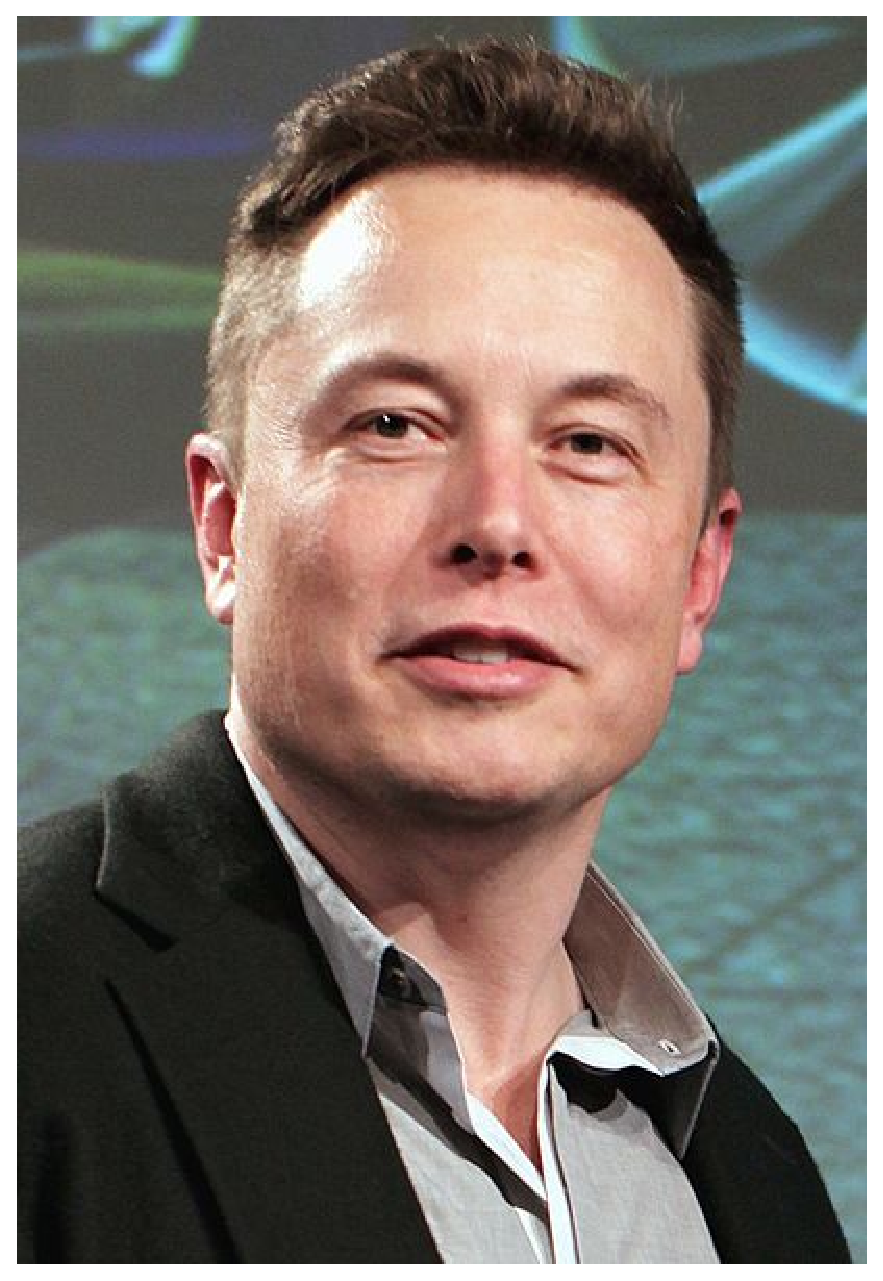
\includegraphics[width=3.5cm]{img/elonmusk.eps}
           \end{tabular}
           & \begin{tabular}{l}
             \parbox{0.5\linewidth}{%  change the parbox width as appropiate
             \textbf{Elon Musk *1971} In 2001 there was a idea of building powerful electric cars by Martin Eberhard and Marc Tarpenning adopted by Elon Musk.}
         \end{tabular}  \\
\end{tabular}
But did they started building electric cars by themselves?
\end{frame}

\begin{frame}{What does 'Scientific working' mean?}
\frametitle{... that needs to be realized by the teams of people}
\begin{figure}
	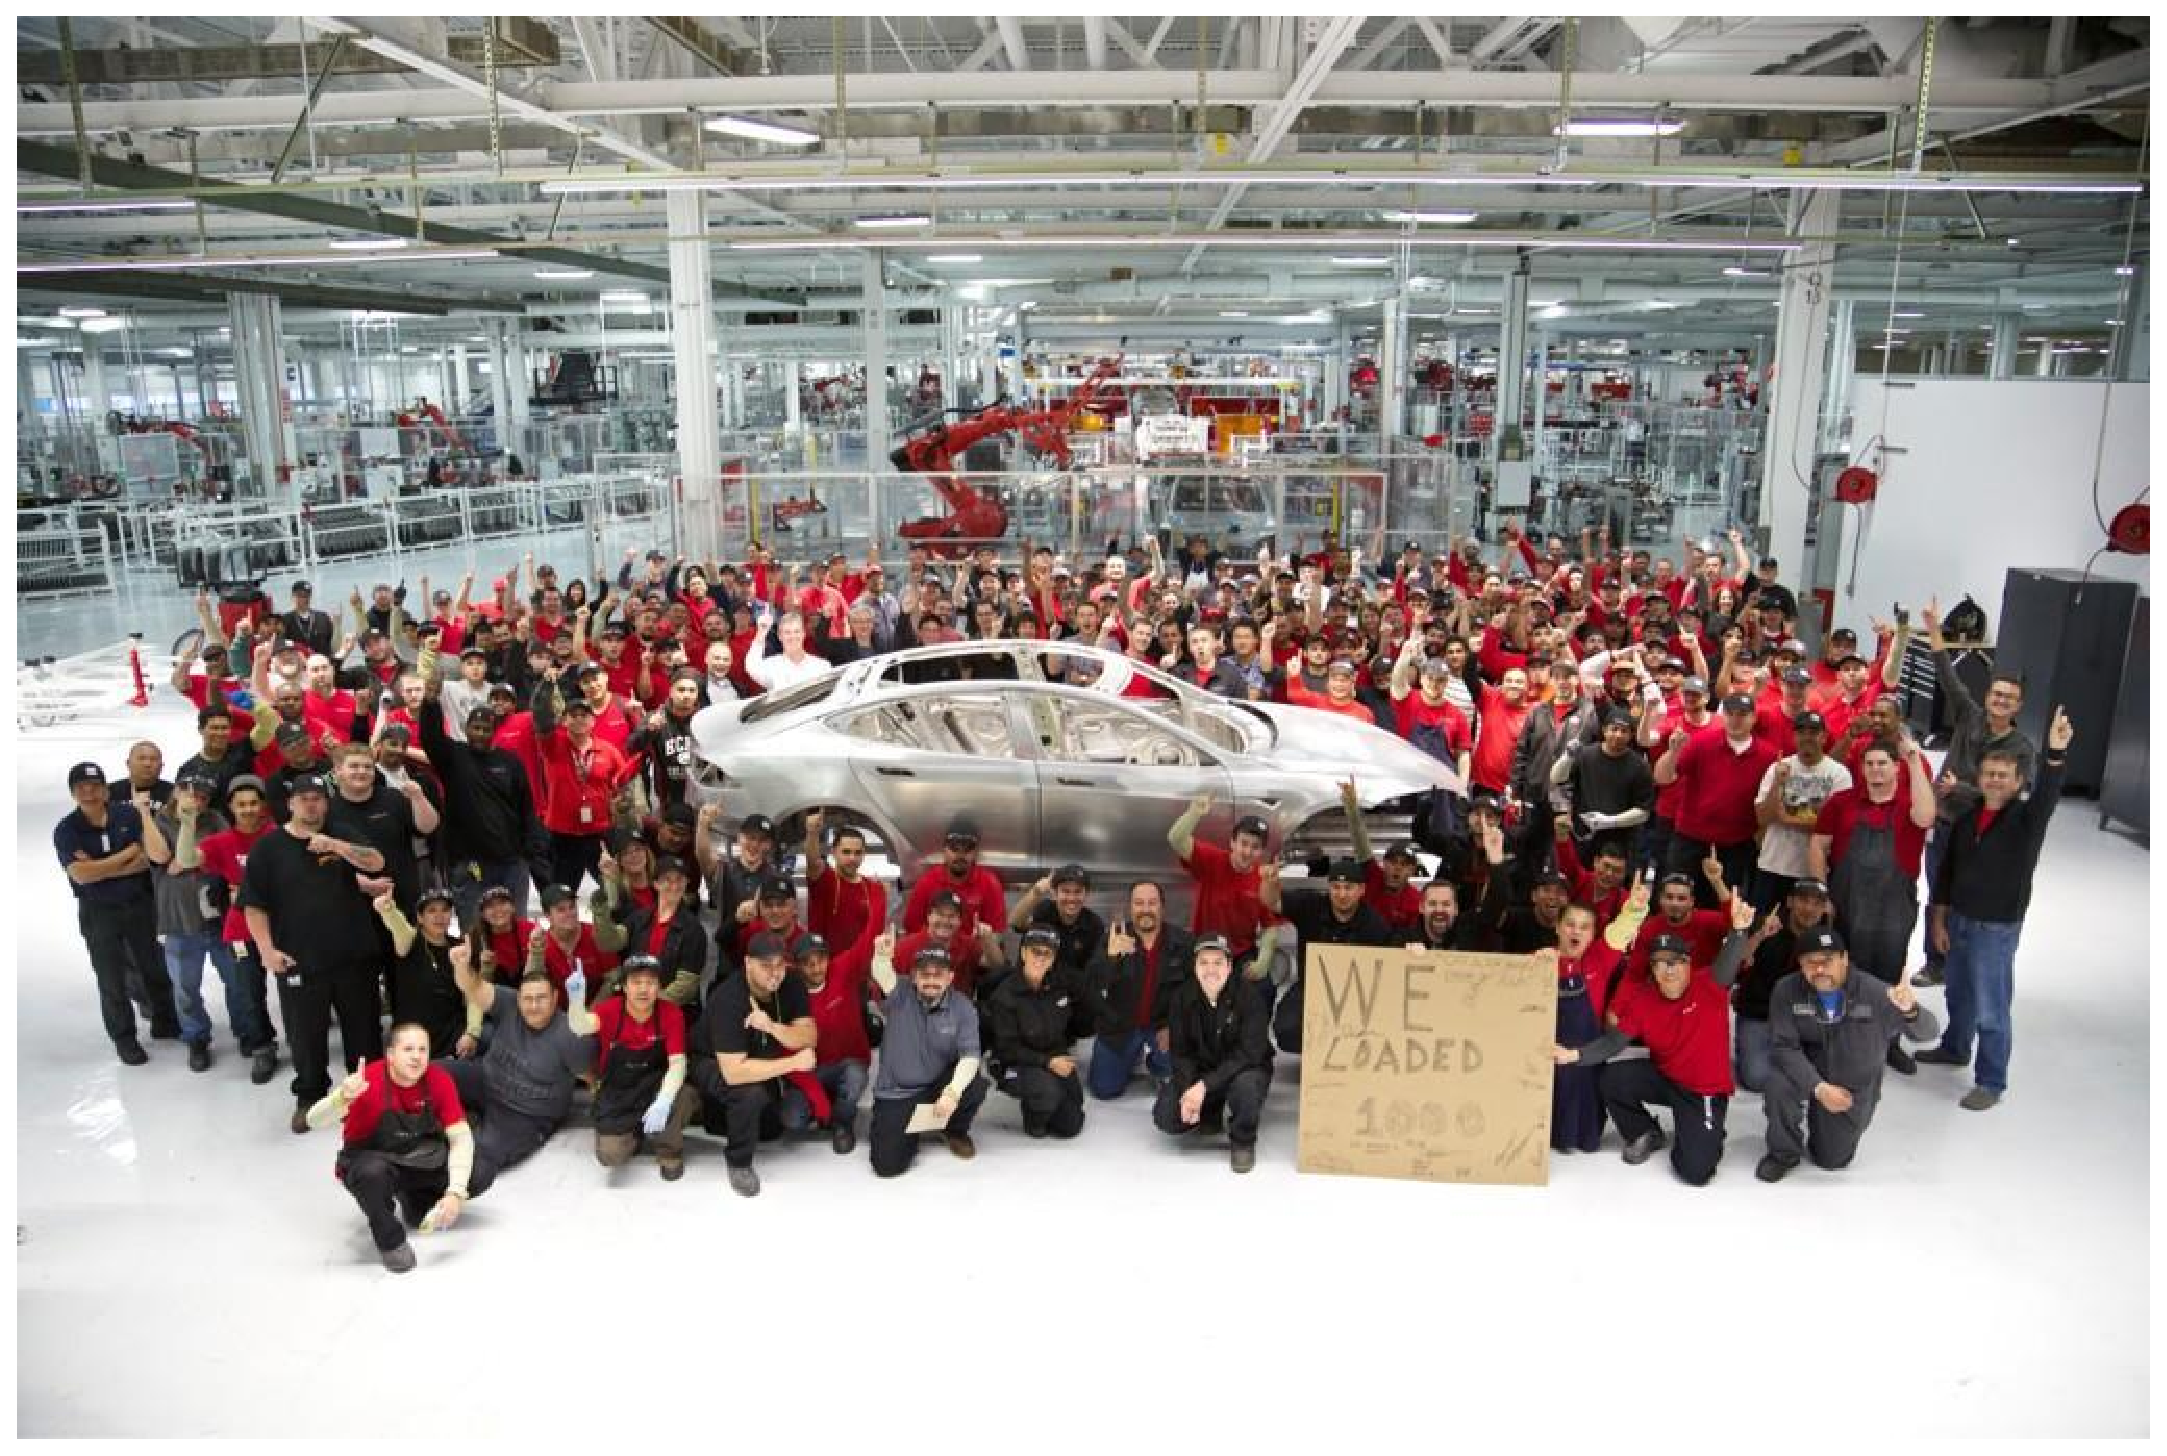
\includegraphics[width=9cm]{img/teslateam.eps}
	\caption{\textcopyright Tesla Inc., source: \href{https://twitter.com/elonmusk/status/262605962005868544}{Twitter account @elonmusk}}
\end{figure}
\end{frame}

\begin{frame}
\textbf{Scientific working is a social discipline that includes}
\begin{itemize}
\item Having great ideas
\item Actually doing own research and science
\item Working in the teams
\item Raising money
\item Publishing papers
\item Giving presentations
\item Evaluating others people work
\end{itemize}
\textbf{This class will streghten your skills in}
\begin{itemize}
\item Giving presentations on scientific topics
\item Working in the teams
\item Evaluating others people work
\end{itemize}
\end{frame}

\begin{frame}
\frametitle{Scientists are evaluated based on their publications}
\begin{itemize}
\item Measurement of quality of publication is a impact factor of the journal (IF)
\item One needs to compare journal impact factors within particular field
\item Medical and economical journals tend to have higher impact factors
\item Better journals have more stricter quality standards
\item Higher impacted journals = higher rejection rate (i.e. 70\%)
\item Well established per-rewiew process
\item Experts in the field evaluates work of the scientists
\item \textbf{Accept, change, reject}
\end{itemize}
\end{frame}

\begin{frame}
\frametitle{Survey of the good journals in Medical engineering}
\begin{table}[]
\centering
\label{my-label}
\tiny{\begin{tabular}{@{}lll@{}}
\toprule
\textbf{Journal}                                            & \textbf{Impact Factor} & \textbf{Proposed by}                        \\ \midrule
\textit{Stroke}                                             & 6.032                  & Sebastian Bannasch                          \\
\textit{NeuroImage}                                         & 5.835                  & Domenico Iuso                               \\
\textit{Medical Image Analysis}                             & 4.188                  & Samuel Manthey                              \\
\textit{\textbf{IEEE Transactions on Medical Imaging}}      & \textbf{3.942}         & \textbf{S. Bannasch, S. Manthey, R. Frysch} \\
\textit{American Journal of Neuroradiology}                 & 3.55                   & Sebastian Bannasch                          \\
\textit{Medical Physics}                                    & 2.617                  & Sebastian Bannasch                          \\
\textit{Physics in Medicine \& Biology}                     & 2.742                  & Domenico Iuso, Robert Frysch                \\
\textit{IEEE Signal Processing Letters}                     & 2.528                  & Robert Frysch                               \\
\textit{Int. J. of Computer Assisted Radiology and Surgery} & 1.863                  & Samuel Manthey                              \\ \bottomrule
\end{tabular}}
\end{table}

\footnotesize{
\begin{itemize}
\item Do your own research
\item Ask for a good journals from your field
\item If you would publish your results, what journal you would have choosen?
\end{itemize}
}
\end{frame}


\section{Committees}
\begin{frame}
\frametitle{Formation of committees}
\end{frame}

\section{Choose paper to present and apply to committee}
\begin{frame}
\frametitle{Choose yor paper to present}
\begin{itemize}
\item Go through the committees proposals
\item Ask your teachers, supervisors
\item Go through the paper suggestions on course webpage
\item Do your own search for a good paper
\item When you choose a paper, apply to the committee.
\item The paper should be in scope of the committee by its proposal.
\item When rejected, choose other committee or contact me.
\item \textbf{Student can not apply to present in his/her own committee.}
\item \textbf{To 23.4.2018 each student have to have per-reviewed paper selected to present.}
\end{itemize}
\end{frame}

\begin{frame}
\frametitle{Acceptance of presenters by committees}
\begin{itemize}
\item Committee must accept the same number of presentation as is the number of its members (quota).
\item Committees will evaluate presenters applications in the order as received by corresponding member.
\item If the quota is not exceeded and someone want to present paper suggested by committee, committee must accept the paper.
\item If someone wants to present already taken paper, commitee rejects the request or suggest another paper.
\item Committee evaluate if particular paper is in its scope and accept or reject the presentation or suggest change.
\item Committee reject all further applications if the quota is exceeded and mail it to the teacher.
\item Committee decide if it accepts/rejects presentation in 3 days.
\item Committee assigns two of its members as reviewers for each presentation.
\end{itemize}
\end{frame}

\section{Per-review process}
\begin{frame}
\frametitle{Per-review process}
\begin{itemize}
\item Each student have to send his or her presentation for a review to 25.5.2018.
\item Sending video for extra point.
\item LaTeX presentation for extra point.
\item Reviewer have three weaks to write a review.
\item 15.6.2018 have to be all reviews submitted.
\item He/she has to describe presentation, identify weak points, suggest improvements.
\end{itemize}
\end{frame}

\begin{frame}
\frametitle{Evaluation of presentation proposals by reviewers}
Reviewer have to suggest that the presentation is:
\begin{itemize}
\item \textbf{Acceptable as is} for the best proposals without any flaws.
\item \textbf{Acceptable after corrections} Reviewer would like to see some improvements or clarifications and after they will be done, talk is acceptable.
\item \textbf{Require improvements} For the presentation that can not be presented as is and needs substantial improvements.
\item \textbf{Require major improvements} For the presentation that lacks essential points and needs to be almost completely rewritten.
\end{itemize}
Reviewer must clearly state which parts of presentation should be rewritten or are in his/her opinion wrong.
\end{frame}


\begin{frame}
\frametitle{Response to reviewer}
Student is obligated to:
\begin{itemize}
\item Respond to the all point by the reviewer.
\item If he or she agrees with a reviewer, correct his or her presentation.
\item If he or she does not agree, explain reviewer why the change is not appropriate.
\end{itemize}
Reviewers might have several rounds of iteration until they decide to accept presentation as is. All reviews and responses must be also send to the class teacher. Final decision is on the class teacher.
\end{frame}

\section{Presentation delivery}

\begin{frame}
\frametitle{Presentation in class}
\begin{itemize}
\item Presentation time is 20 minutes
\item Discussion for 10 minutes
\item Three presentations for the class
\item Typical class will contain presentations of a single comittee
\item Reviewers will evaluate also final presentation and its delivery
\item Committee members will moderate the class of the commitee
\item Committee is responsible for setting order of presentations in the class
\end{itemize}
\end{frame}

\begin{frame}
\frametitle{Best practices}
\begin{itemize}
\item 20 minutes can be coverred by around 15 slides
\item Think about rhetorical situation
\item Consider enrollment into the public speaking course
\item Think about invention, arrangement, style, memory and delivery
\item Presenter should know the paper well and be prepared for a discussion
\item Reviewers should also know the paper well and be prepared as well
\end{itemize}
\end{frame}

\begin{frame}
\frametitle{Poor practices}
\begin{itemize}
\item Extensive use of copy/paste might be considered as plagiarism leading to not being clasified
\item Moderate text content of the slides
\item Presentation without illustrations
\item Presentation without introduction or summary
\item Hardly understandable presentations for non experts in the topic
\item Not citing all resources might be considered plagiarism as well
\end{itemize}
\end{frame}

\begin{frame}
\frametitle{Evaluation - invention}
\begin{itemize}
      \item{Paper was in the scope of the class and lesson (medical engineering)}
      \item{Paper was sufficiently complex for the class}
      \item{Presentation well addresses also the audience without a deep knowledge of the topic}
\end{itemize}
\end{frame}

\begin{frame}
\frametitle{Evaluation - arrangement}
\begin{itemize}
      \item{Is the talk structured in the meaningful and logical way?}
      \item{Was the proper introduction to a topic given?}
      \item{Was the proper conclusion given? Were there summarized clearly important parts of the talk?}
\end{itemize}
\end{frame}

\begin{frame}
\frametitle{Evaluation - style}
\begin{itemize}
      \item{The style of the presentation adds up to the understandability of the topic.}
      \item{Proper incomporation of image/media into the presentation.}
      \item{Meaningful captions of the figures}
      \item{Correct references and citations}
      \item{Use the template of OVGU university.}
\end{itemize}
\end{frame}

\begin{frame}
\frametitle{Evaluation - memory}
\begin{itemize}
      \item{Presenter was well prepared for the talk and the flow of the presentation was smooth.}
      \item{Free speach without major support of manuscript.}
      \item{Compliance with a duration of 20 minutes (2 min. tolerance).}
\end{itemize}
\end{frame}

\begin{frame}
\frametitle{Evaluation - delivery}
\begin{itemize}
      \item{Good contact and communication with the audience.}
      \item{Posture towards the audience, proper gestures.}
      \item{Speach clarity, articulation, sufficient speach level.}
\end{itemize}
\end{frame}

\begin{frame}
\frametitle{Evaluation - discussion/other}
\begin{itemize}
      \item{Was the presentation without factical mistakes?}
      \item{Does the presentation provide correct explanation of the main results of the presented paper?}
      \item{Was the speaker well prepared for the discussion?}
\end{itemize}
\end{frame}


\begin{frame}
\frametitle{Evaluation - feedback and questions}
\begin{itemize}
\item Learn how to ask.
\item Asking in the course is a required activity.
\item Try to help presenter to improve by your questions.
\item Committee members should ask.
\item Reviewers should also give feedback on progress during review process.
\end{itemize}
\end{frame}

\section{Summary}
\begin{frame}
\frametitle{Summary of the class assignments}
\begin{itemize}
\item You will learn how to interact in the peer review process
\item You will form 3 people committees that resemble journal boards (to 16.4.2018)
\item You will apply to a commitee for presentation (to 23.4.2018)
\item You will create your presentation and send it for review (to 25.5.2018)
\item You will review presentations of two other people (to 15.6.2018)
\item You will improve your presentation based on the reviews
\item You will deliver your presentation in the class ... next semester
\end{itemize}
\end{frame}



\begin{frame}
\frametitle{Thank you for your attention, looking forward to your presentations.}

\textbf{Contact}

Vojt\v{e}ch Kulvait

\textit{Room} G09-319

\textit{E-mail} \href{mailto:vojtech.kulvait@ovgu.de}{vojtech.kulvait@ovgu.de}


\textbf{Course webpage}

\url{https://elearning.ovgu.de/course/view.php?id=637}
\end{frame}

\end{document}
